\documentclass[sigchi]{acmart}
\usepackage{graphicx} % Required for inserting images
\usepackage[fencedCode]{markdown}
\graphicspath{ {./images/} }

% defining the \BibTeX command - from Oren Patashnik's original BibTeX documentation.
\def\BibTeX{{\rm B\kern-.05em{\sc i\kern-.025em b}\kern-.08emT\kern-.1667em\lower.7ex\hbox{E}\kern-.125emX}}

% end of the preamble, start of the body of the document source.
\begin{document}

\title{Are you more “proukr” o “dontcare”? 
What a hashtag can say about you}

\author{Gufa}
\email{gufeggio@unipi.it}
\affiliation{%
  \institution{Student ID: cruu cruuuu}
}

\author{Davide Perra}
\email{d.perra@studenti.unipi.it}
\affiliation{%
  \institution{Student ID: 616686}
}

\author{Fabio Michele Russo}
\email{f.russo11@studenti.unipi.it}
\affiliation{%
  \institution{Student ID: 429892}
}

\renewcommand{\shortauthors}{Diamanti, Perra, Russo}

% This command processes the author and affiliation and title information and builds
% the first part of the formatted document.
\maketitle

\markdownInput{ch012.md}

\begin{figure}[h]
\caption{xxx caption 1, 2, 3}
\centering
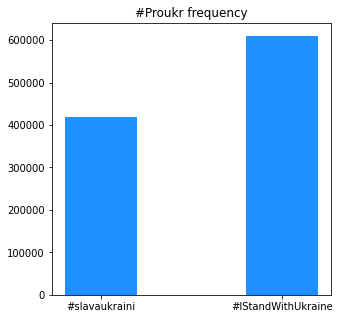
\includegraphics[width=0.15\textwidth]{intro_11}
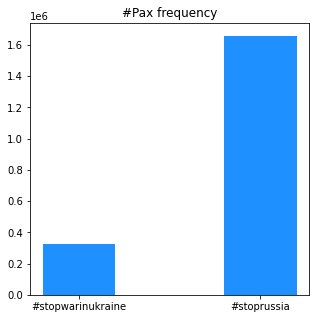
\includegraphics[width=0.15\textwidth]{intro_12}
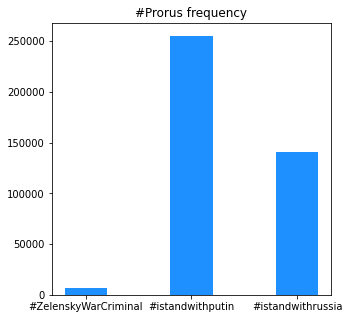
\includegraphics[width=0.15\textwidth]{intro_13}
\end{figure}

Finally, among the most popular hashtags we selected the three, one for each category, which had a frequency as similar as possible. The table below shows our choice with the respective counts:

xxx table 1

\markdownInput{ch012b.md}

$$\text{support} = \frac{\text{(number of tweets in which the hashtag appears)}}{\text{(total number of tweets obtained by our query)}}$$

and we define threshold\_support = 0.9/10000, a number manually set as the minimum reasonable fraction of tweets in which a hashtag must appear to be included in the categorization phase. 
For a hashtag to be considered it must have 

$$support \geq threshold\_support$$

\markdownInput{ch012c.md}

xxx img 4

\markdownInput{ch012d.md}

$$max(scores) \geq 1.2 * median(scores)$$

\markdownInput{ch012e.md}


\begin{figure}[h]
\caption{xxx wordclouds 1, 2, 3}
\centering
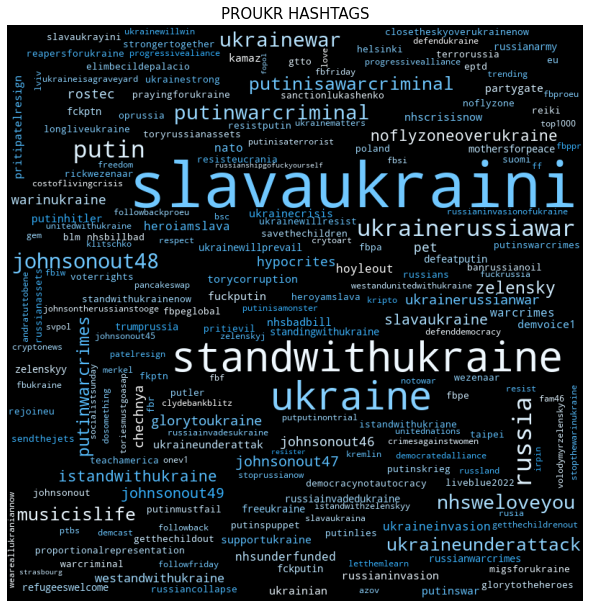
\includegraphics[width=0.15\textwidth]{intro_21}
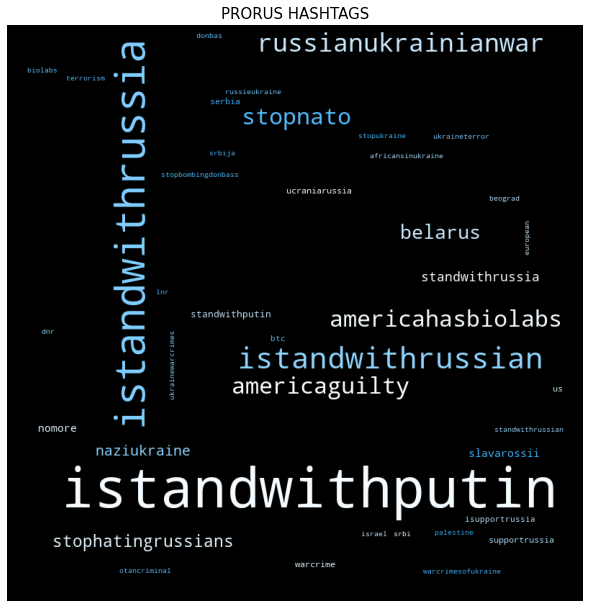
\includegraphics[width=0.15\textwidth]{intro_22}
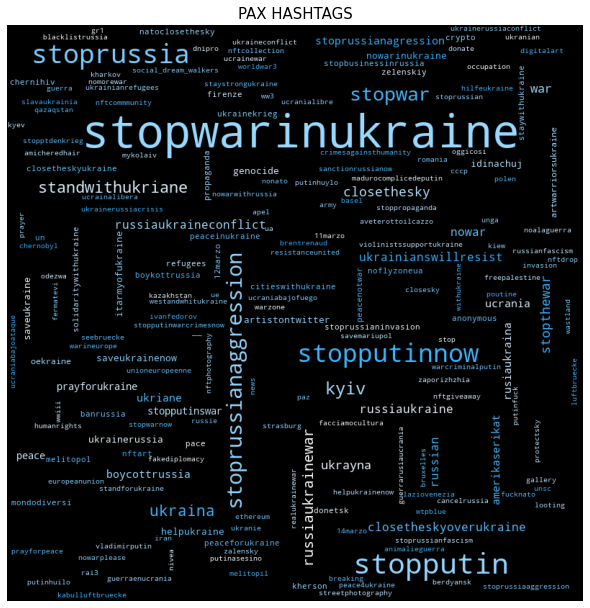
\includegraphics[width=0.15\textwidth]{intro_23}
\end{figure}

\markdownInput{ch012h.md}

\markdownInput{ch3.md}

xxx table 1
xxx image 1

\markdownInput{ch3b.md}

xxx table 2

\markdownInput{ch3c.md}

xxx table 3

\markdownInput{ch3d.md}

xxx image 2

\markdownInput{ch3e.md}

xxx image 3
xxx image 4

\markdownInput{ch3f.md}

xxx table 3

\markdownInput{ch3g.md}

xxx image 5

\markdownInput{ch3h.md}

xxx table 4

\markdownInput{ch3i.md}


\markdownInput{ch3l.md}


\markdownInput{ch45.md}

\begin{figure}[h]
\caption{xxx heatmap}
\centering
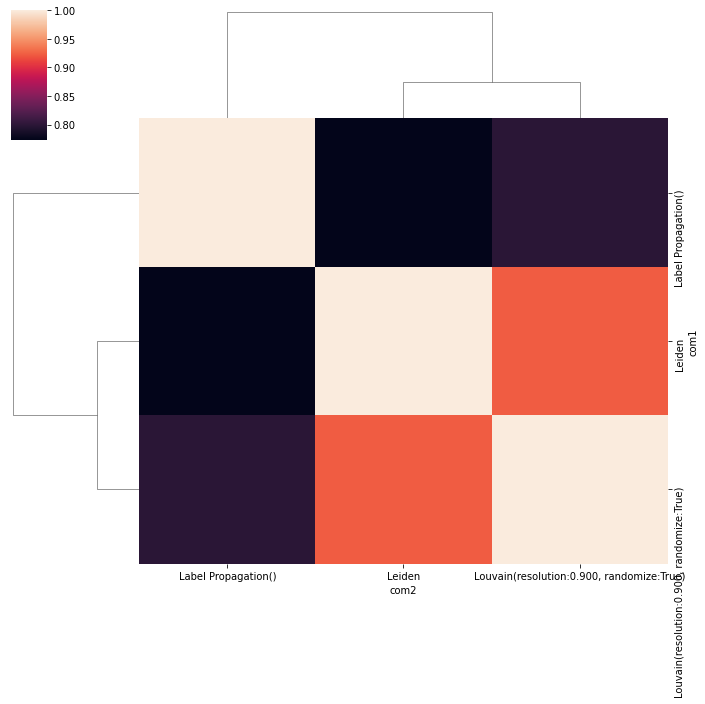
\includegraphics[width=0.45\textwidth]{static_community_discovery}
\end{figure}

\markdownInput{ch45c.md}

\markdownInput{ch6.md}

- $t_0$: From 15/02 to 15/03 we observe the opinions in the month straddling the date of the outbreak of the war. This is the time period spent so far in this work and the network generated previously.
- $t_2$: From 15/04 to 15/05 we observe opinions about two months after the start of the war. We observe the same users we observed in t0 and re-categorize them in t2 according to their opinions in this later time period. Categorization is done in the same way as for t0, as already reported in chapter 2.

These are the Transition Matrix and the representation of the Markov Chain.

\begin{figure}[h]
\caption{xxx 2 immagini open question}
\centering
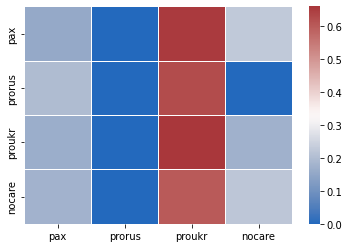
\includegraphics[width=0.23\textwidth]{open_question_1}
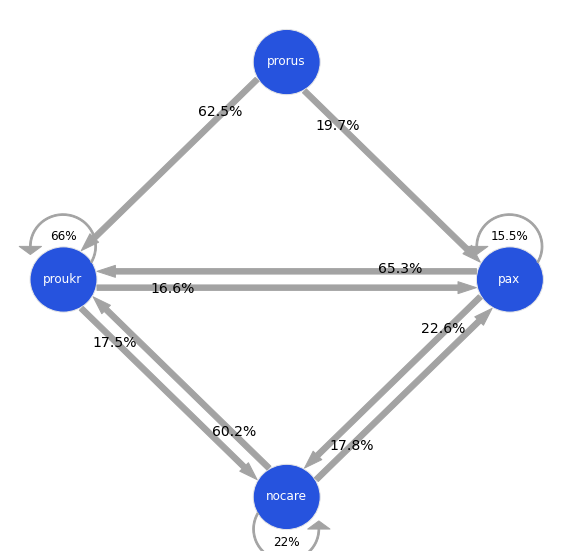
\includegraphics[width=0.23\textwidth]{open_question_2}
\end{figure}

\markdownInput{ch6d.md}

- $t_1$ = 15-03-2023 / 15-04-2023, a time interval captured to understand what happens between the beginning of the war ($t_0$) and two months later ($t_2$)

The line chart below shows how the sum total of all opinions for each category changes from $t_0$ to $t_2$.

\begin{figure}[h]
\caption{xxx line chart}
\centering
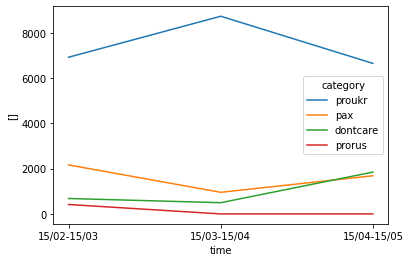
\includegraphics[width=0.45\textwidth]{open_question_3}
\end{figure}

\markdownInput{ch6e.md}

\begin{figure}[h]
\caption{xxx albero open question}
\centering
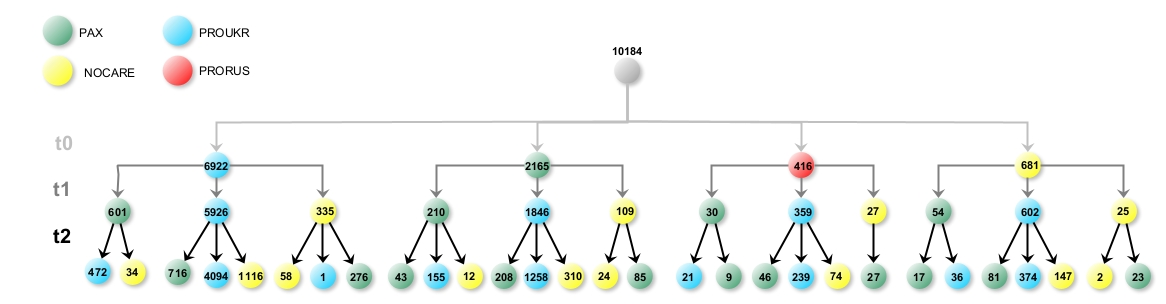
\includegraphics[width=0.45\textwidth]{open_question_4}
\end{figure}

\markdownInput{ch6g.md}



% The next two lines define the bibliography style to be used, and the bibliography file.
\bibliographystyle{ACM-Reference-Format}

\end{document}
